\chapter{Blended GTL fuel models}

\section{GTL fuel composition}


Synthetic jet fuels have become an area of increasing interest, in order to curb the emissions and pollution levels in air transportation dependent on conventional oil-derived jet fuels \cite{RePEc:eee:energy:v:43:y:2012:i:1:p:111-123}. As a result of this interest as well as mission to reduce the over-dependence on conventional oil-derived fossil fuels and reduce carbon footprint, future designs of aero-propulsion engines will rely on the computational modeling of sustainable and alternative jet fuels \cite{Corporan2007EmissionsFuel}\cite{Hermann2006ChemicalFuel}. Chapter 1 and 2 has gone in detail on the need for the computational modeling of jet fuel as well as jet fuel fuel surrogates. Since, predictions of jet fuel combustion kinetics is central to the fuel reactivity in aero-propulsion engines, parameters such as auto-ignition properties of the fuel surrogates is necessary to understand its behavior under engine-like conditions. 

The most common parameter used is the ignition delay time and it is heavily dependent on the combustion kinetics as well as the macroscopic characteristics of temperature, pressure and mixture composition fractions of the fuel. Jet fuels typically contain thousands of both major and minor constituents and as such modeling a real jet fuel is not viable due to the complexity as well as computational resources required. The use of surrogate models are applicable based on the major constituents of the jet fuel, where the physical properties are carefully chosen to match the physical characteristics of the fuel and that of the chemical properties tested and modeled under carefully chosen conditions \cite{Edwards2001SurrogateFuels}\cite{Huber2008SurrogateCurve}. While all of this major aspects of surrogate models have been covered in chapter 2, more emphasis is laid in this chapter on the constituents of various alternative jet fuels and specifically on F-T GTL fuel blend mixtures.


\vspace{2cm}


Experimental investigation of alternative jet fuel includes ignition delay time measurements in shock tubes and rapid compression machines (RCM) \cite{Dean2007AutoignitionPressures}\cite{Wang2012}\cite{Malewicki2013ExperimentalN-dodecane}\cite{Dagaut2014}\cite{Dagaut2014CombustionModeling}\cite{Dagaut2016ExperimentalSurrogates}\cite{Askari2016}\cite{Valco2016LowMachine}, laminar flame speeds \cite{Singh2011ExperimentalFlames}\cite{Wang2012}\cite{Hui2013LaminarPressures}\cite{Dagaut2014}\cite{Yu2016TheoreticalFuel}, chemical structure from pyrolysis and oxidation in pressure flow reactors as well as oxidation in a jet stirred \cite{Gokulakrishnan2007ExperimentalConditions}\cite{Gokulakrishnan2008IgnitionFuel}\cite{Honnet2009AKerosene}\cite{Dooley2010AProperties}\cite{Mze-Ahmed2010KineticsStudy}\cite{Dagaut2014CombustionModeling}\cite{Dagaut2014}\cite{Dagaut2015TheStudy}\cite{Dagaut2016ExperimentalSurrogates}, emissions in a gas turbine combustor rig \cite{Hermann2006ChemicalFuel}. These experimental measurements provide a basis with which to compare chemical kinetic models of jet fuel surrogates as a means of validating the mechanisms. 

Similarly, several kinetic models of jet fuel surrogates have been published over the years using the chemical kinetic mechanism generation code PSR \cite{Glarborg1986PSR:Reactors} a Fortan solver for simulating well-stirred reactors used by Mzé-Ahmed and others in the mechanism of a synthetic jet fuel \cite{Mze-Ahmed2010KineticsStudy}, models have also been published on F-T synthetic surrogate fuels using the CHEMKIN suite code from Naik et al \cite{Naik2011DetailedFuels}, F-T GTL surrogate models have also been deduced based on surrogate modeling of jet aviation fuels using a three-component fuel surrogate model of n-decane, iso-octane and toluene as described by Dooley et al \cite{Dooley2010MethylModel}. Ranzi et al. followed up with a more compact model of jet fuel model up to \ce{C_16} \cite{Ranzi2012HierarchicalFuels} with more than 8000 reactions and more than 250 species. Although, skeletal models of GTL models have been built in the past by Dagaut et al \cite{Dagaut2014}, more recently, Dagaut et al \cite{Dagaut2016ExperimentalSurrogates} built a detailed model of a GTL mechanism with 3 components with more than 10000 reversible reactions and more than 2000 species. The reaction pathways of these models are representive of the individual PRFs used in the mechanism generation.


The GTL fuel composition was based on the composition as defined by Dagaut et al in the work on the experimental and modeling of GTL fuel surrogates \cite{Dagaut2014}. The summary of the GTL fuel surrogate used in this work and the comparison to the real fuel is in table \ref{tab:GTL_model_summary}.


\begin{table}[ht]
\arrayrulecolor[HTML]{DB5800}
\caption{Summary of RMG GTL fuel surrogate model composition}
\centering
\begin{adjustbox}{width=1\textwidth}
\begin{tabular}{ p{6cm} c c c c c }
\rowcolor{lightgray}\multicolumn{5}{|c|}{RMG iso-octane model summary} \\
 Fuel &  Fuel composition &  (\% weight) & Fuel properties & Experimental conditions \\
 GTL & \begin{tabular}{ c }
    n-Paraffins:  \\ 
    iso-Paraffins \\
    di-Naphthenes \\
    mono-Naphthenes \\ 
    Aromatics \\
 \end{tabular} & \begin{tabular}{ c } 
       28.1 \\
      62.8  \\
     8.2 \\
     0.6 \\
     0.2 \\
 \end{tabular} & \begin{tabular}{ c }
      \ce{C_{10.45}H_{23.06}}  \\
       Hydrogen-Carbon ratio (H/C) : 2.20 \\
      Cetane Number (CN): $58.0^a$ \\
       Density $\rho$: 737 g/L \\
 \end{tabular} & \begin{tabular}{ c }
      $\phi = 1.0$  \\
      Temperature range: 560 - 1110 K \\
      10,450 ppm of C \\
 \end{tabular} \\ 
 \hline 
 GTL Surrogate & \begin{tabular}{ c }
      n-decane  \\
      iso-octane \\
      n-propyl-cyclohexane \\
 \end{tabular} & \begin{tabular}{ c }
      57.7  \\
      33.2 \\
      9.1 \\
 \end{tabular} & \begin{tabular}{ c }
      $\ce{C_{10.45}H_{22.95}}^a$ \\
      Hydrogen-Carbon ratio (H/C) : 2.1966 \\
      Derived Cetane Number (CN): 54.5 \\
       Density ($\rho$) at $15^{\circ}C$: 723 g/L \\
       Molar weight $148.31^a$ g/mol \\
       \hline
       $^a 1.13\times \ce{C_{9.2451}H_{20.308}}$ since 1130 ppm of model fuel was used to present 1000 ppm of GTL
 \end{tabular} & \begin{tabular}{ c }
      $\phi = 1.0$  \\
      Temperature range: 560 - 1110 K \\
      10,450 ppm of C \\
 \end{tabular} \\
 \end{tabular}
    \end{adjustbox}
    \label{tab:GTL_model_summary}
\end{table}

Kinetic models of jet fuels in previous studies in summarized in table \ref{tab:GTL_model_summary} while the path flux diagram of the GTL model fuel blend is show in fig.\ref{fig:gtl-pfa}





\subsection{Model validation of F-T GTL surrogate fuel model in shock tubes for ignition delay time predictions}

Shock tubes essentially devices designed to experiment and study the flow of high-temperature and high-velocity effects of compressible gases within an actual engine-like environment. It is designed on the basis of knowledge of gas dynamics and analysing shock waves. It operates on the principle that at high temperatures, supersonic gases flow is in the tube a diaphragm causes a separation into regions of high-pressure and low-pressure. As the pressure rises, an unsteady rarefied wave passes into the driver gas with a velocity usually a few kilometers per second causing flow from the high-pressure region to the low-pressure region. As the shock wave progresses in the low-pressure region, it pushes the low-pressure gas ahead of it. Thus, creating two fronts, flow ahead of the shock wave and flow behind the shock wave. The flow ahead of the behind the shock wave (driver gas) is the gas of interest. The velocity of the driver gas is equal to  that of the driven gas\cite{Greene1964TheR.}. Usually, there in the high-pressure region, is an explosive gas which is the gas studied, and present is a laser beam to detect the luminescence of some excited species. The ignition delay time can be defined as the time it takes:
\begin{enumerate}
    \item For the shock wave to hit the wall and propagate with the excitation of a \ce{CH*} or \ce{OH*}radical
    \item For the shock wave to hit the wall and measurement of the highest peak of the temperature in the driven section
    \item For the shock wave to hit the wall and detection of the highest peak of the pressure in the driven section
\end{enumerate}
Since all three possibilities of measuring the ignition delay time data in shock tubes exist, it is often well defined based on one of the three main possibilities usually for the first-stage ignition \cite{Davidson2004InterpretingData}\cite{Fieweger1994Shock-tubePressures}\cite{Fieweger1997Self-ignitionPressure}\cite{Pfahl1996Self-ignitionConditions}\cite{Haylett2012IgnitionTube}

In Cantera, this process is often defined based on the reactor type of interest. First, the gas solution object is created with the \textbf{gas.Solution} class, then a reactor type is selected with the appropriate initial conditions usually coming from the experimental data being validated against. Next, the state of the system is set with the reactor network previously defined and then a simulation in time for the next states is found using the ODE solver. The ODE solver starts at the current state  of the systems and progresses in time by one of the following methods:
\begin{enumerate}
    \item \textbf{step()}: This involves a reactor step from the current state of the system by solving the previous state of the system using the time step given. This is an explicit method where the ODE solver internally solves the numerical Differential Algebraic Equations (DAE) system. The new time is returned as well as the state of the system at the next state using the previously defined time step $\Delta$t within the solver absolute and relative tolerances. The time step cannot be larger than the maximum time step or else the ODE solver breaks.
    \item \textbf{advance($t_{new}$)}: This method solves the state of the system at a predefined step times $t_{new}$. This $t_{new}$ describes the absolute time of the system from the initial system by calling the ignition delay time function for the reactor in a loop, either a while loop or for loop at exactly the time specified - basically using the \textbf{step():} function several times in the process. In addition, the \textbf{advance():} function can be made to continue until a steady-state solution is attained by time stepping. Only when the feature-scaled residual of the state vector is below a given threshold value is the system at steady-state and the ODE solver stops.
\end{enumerate} 
For all shock tube models in this work, a zero-dimensional homogeneous closed ideal gas reactor with constant volume and internal energy class was used since at constant volume, there is no P-V work done against the control volume of the gas. Since the temperature is known, the energy equation is computed assuming adiabatic conditions in the reactor volume. The time integration of the species is computed in uniform time steps until the solution is found. During the time integration, the reactor model scheme usually an ODE SUNDIALS solver \cite{hindmarsh2005sundials} solves the differential equations of the species within the energy equation. The energy equation accounts for the energy interaction via the heat equation but is ignored since the reactor assumes adiabatic conditions and indicates only mechanical work interactions, mass transport due to species diffusion and conversion.  The equation being solved in the ideal gas reactor  of Cantera is equation \ref{eq.mass conservation} as given by Robert Kee et al's book on Chemically Reacting Flow \cite{Kee2003ChemicallyPractice}. The definition of the ignition delay time varies. Nonetheless, the model used in Cantera assumes an ignition delay time based on the excited \ce{CH} or \ce{OH} radical species and is often very close to the highest temperature spike Ji et al point out for the sensitivity analysis of ignition delay times \cite{Ji2019EvolutionAutoignition}. 

\begin{equation}
    U = m\sum_k{Y_k u_k(T)}
\end{equation}

\begin{equation}
    \frac{dU}{dt} = u\frac{dm}{dt}+mc_v\frac{dT}{dt}+m\sum_k{u_k \frac{dY_k}{dt}}
\end{equation}

\[\text{Substituting the corresponding derivations for temperature in the reactor as:} \]


\begin{equation}
    mc_v\frac{dT}{dt}=-p\frac{dV}{dt} - Q^. + \sum_{in}{m_{in}(h_{in}- \sum_k{u_k Y_{k, in}}) -\frac{pV}{m}\sum_{out}{m_{out}^.} - \sum_k{m_{k, gen}^. u_k}}
    \label{eq.mass conservation}
\end{equation}

The ignition delay times prediction are presented as modeled in Cantera against shock tube experiments of Wang et al.\cite{Wang2012}.

\begin{table}[ht]
\arrayrulecolor[HTML]{DB5800}
\caption{Summary of kinetic mechanisms of jet fuel surrogates composition}
\centering
\begin{adjustbox}{width=1\textwidth}
\begin{tabular}{ p{6cm} c c c c c }
\rowcolor{lightgray}\multicolumn{5}{|c|}{RMG iso-octane model summary} \\
 Fuel &  Surrogate fuel model composition &  (\% composition) & kinetic model species and reactions & Reference \\
 \hline
 GTL synthetic paraffinic kerosene (SPK) & \begin{tabular}{ c }
      n-decane  \\
      iso-octane \\
      n-propyl-cyclohexane \\
 \end{tabular} & \begin{tabular}{ c }
      57.7  \\
      33.2 \\
      9.1 \\
 \end{tabular} & Low temperature and high temperature mechanism; 1876 species and 23127 reactions & Current Study \\
 \hline
 Jet A & \begin{tabular}{ c }
    n-decane \\
    iso-octane \\
    toluene \\
 \end{tabular} & \begin{tabular}{ c } 
       42.67 \\
      33.02  \\
      24.31 \\
 \end{tabular} & Low temperature and high temperature mechanism; 753 species and 9980 reactions without PAH mechanism & Dooley et al. \cite{Dooley2010AProperties} \\
 \hline 
 S-8 & \begin{tabular}{ c }
      n-decane  \\
      iso-octane \\
      n-dodecane \\
 \end{tabular} & \begin{tabular}{ c }
      25.0  \\
      32.0 \\
      43.0 \\
 \end{tabular} & High temperature mechanism; 597 species and 4668 reactions & Naik et al. \cite{Naik2011DetailedFuels}\\
 \hline
 Shell GTL & \begin{tabular}{ c }
      n-decane  \\
      iso-octane \\
      n-dodecane \\
 \end{tabular} & \begin{tabular}{ c }
      61.0  \\
      28.0 \\
      11.0 \\
 \end{tabular} & High temperature mechanism; 597 species and 3854 reactions & Naik et al. \cite{Naik2011DetailedFuels}\\
 \hline
 GTL synthetic paraffinic kerosene (SPK) & \begin{tabular}{ c }
      n-decane  \\
      iso-octane \\
      n-propyl-cyclohexane \\
 \end{tabular} & \begin{tabular}{ c }
      65.2  \\
      37.5 \\
      10.3 \\
 \end{tabular} & Low temperature and high temperature mechanism; 2182 species and 8347 reactions & Dagaut et al. \cite{Dagaut2014} \\
 \end{tabular}
    \end{adjustbox}
    \label{tab:GTL_model_summary}
\end{table}



As seen in fig. \ref{fig:gtl-blend-idt}, there is close agreement at to experiments of Wang et al.\cite{Wang2012} who studied three jet fuels, conventional jet fuels Jet A and JP 8, two F-T GtL fuels, S-8 and Shell GtL and one F-T coal-to-liquid Sasol IPK under engine-like conditions in a shock tube using the chemiluminescence of \ce{OH^*} radicals for the ignition delay time measurement of the jet fuel mixtures with air for $\phi=1.0$ at 20 atm. The NTC regime of the RMG model of the GTL fuel surrogate is not as pronounced and a sensitivity analysis would aid knowing which reactions are most sensitive to the onset of ignition in the low temperature mechanism region.


\begin{figure}[hbp]
    \centering
    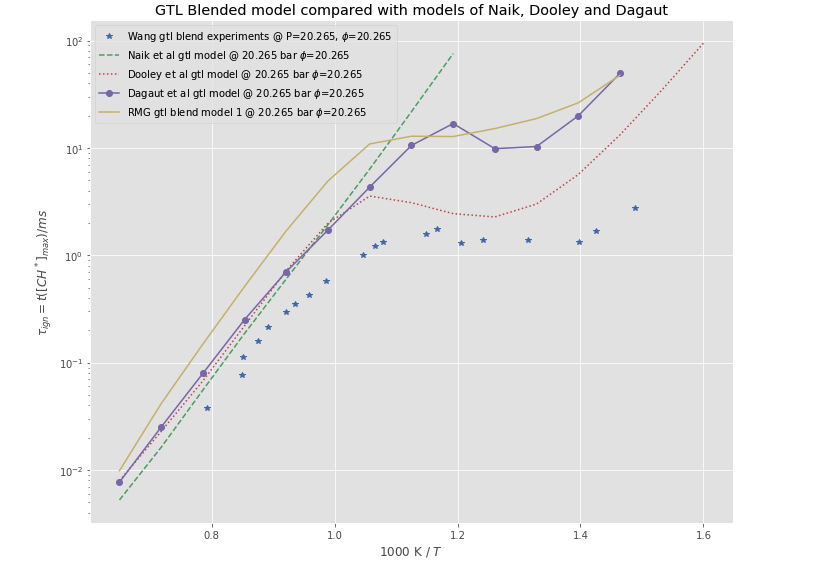
\includegraphics[scale=0.5, keepaspectratio]{images/GTL_model_blend_idt.png}
    \caption{Ignition delay times of GTL cross-reacted fuel blend with models of Naik et al. \cite{Naik2011DetailedFuels}, Dooley et al. \cite{Dooley2010AProperties}, Dagaut et al. \cite{Dagaut2014} compared against shock tube experiments of Wang et al. \cite{Wang2012} at 20 atm and stoichiometric conditions with air. Lines represent model predictions and symbols experimental measurements}
    \label{fig:gtl-blend-idt}
\end{figure}